\documentclass[10pt,letterpaper]{article}
\usepackage[margin=0.65in,headheight=14pt]{geometry}
\usepackage[T1]{fontenc}
\usepackage{lmodern,microtype,amsmath,amssymb,booktabs,array,graphicx,xcolor,hyperref,fancyhdr,enumitem}
\definecolor{ink}{HTML}{24517E}
\hypersetup{colorlinks=true,urlcolor=ink,linkcolor=ink,pdftitle={N=8 and N=10 spheres with projected edge confinement},pdfauthor={Research note},pdfsubject={Model, exact convergence diagnostics, and no-edge comparisons}}
\graphicspath{{n8_edge_note/}}
\setlength{\parindent}{0pt}
\setlength{\parskip}{4pt}
\setlength{\abovedisplayskip}{5pt}
\setlength{\belowdisplayskip}{5pt}
\setlength{\emergencystretch}{2em}
\setlist{nosep,leftmargin=1.25em}
\renewcommand{\arraystretch}{1.08}
\pagestyle{fancy}\fancyhf{}
\fancyhead[L]{\small N=8 and N=10 FQHE with SPRING}
\fancyhead[R]{\small Projected edge confinement}
\fancyfoot[L]{\footnotesize Experiment note \textbullet\ Updated 10 November 2026}
\fancyfoot[R]{\thepage/3}
\newcommand{\topic}[1]{\vspace{3pt}\textbf{\color{ink}#1}\par}
\newcommand{\fid}{\mathcal F}
\newcommand{\de}{\delta E}
\newcommand{\V}{V_1}
\begin{document}
\begin{center}
{\Large\bfseries N=8 and N=10 Spheres with Edge Confinement}\\[3pt]
{\large Model, numerical outcome, and comparison with no confinement}
\end{center}

The $N=8$ matched pilot learns its modified confined ground state more effectively than the unconfined cap. Its tabulated continuations reach 92.74\% fidelity. The new $N=10$ calculation reaches 57.07\% fidelity after 130,000 total updates on the local RTX 4070 Ti SUPER. Both retain finite exact energy error. Finite-batch effects have controlled support in one $N=8$ trajectory; projected wall broadening remains an untested contributor to incomplete convergence.

\topic{1. Geometry, conventions, and Hamiltonian}
We retain $N$ spin-polarized fermions in the lowest Landau level (LLL) of the Haldane sphere. Write the flux as $F=2Q$. Two extra flux quanta give the north-pole Laughlin cap room for an edge: $F=3(N-1)+2$. Our convention is
\[
 \phi_k\propto u^{F-k}v^k,\quad m_z=F/2-k,\quad
 K=\sum_k k n_k=\tfrac32N(N-1),\quad L_z=NF/2-K=N.
\]
Larger $k$ lies farther south; the code index is $a=F-k$. With $\hbar=1$, both sizes retain all $F+1$ orbitals and the complete fixed-$K$ sector:
\begin{center}\small
\begin{tabular}{@{}rrrrrrr@{}}\toprule
$N$ & $F$ & Orbitals & $K$ & $L_z$ & Sector states & Real parameters\\\midrule
8 & 23 & 24 & 84 & 8 & 15,744 & 1,730\\
10 & 29 & 30 & 135 & 10 & 473,259 & 2,114\\\bottomrule
\end{tabular}
\end{center}
The Hamiltonian is
\begin{equation}
 H=\V\sum_{i<j}P_{ij}(R=1)+\sum_{k=0}^{F}\epsilon_k n_k,
 \qquad \alpha L^2=0.
 \label{eq:H}
\end{equation}
Here $P_{ij}(R=1)$ is the normalized relative-pair-angular-momentum-one projector; $V_3=0$. Confinement preserves $L_z$ but breaks full rotational symmetry. Ground-state statements concern each specified sector; other $K$ sectors were not compared.

\topic{2. Why use $U(x)=10\V\Theta(x-0.88)$?}
Here $\Theta$ is the Heaviside function, $\theta$ is polar angle, and $x=\sin^2(\theta/2)$. The wall penalizes the southern 12\% of sphere area, beyond $\theta_c=139.46^\circ$. Its illustrative cutoff equals the mean position of the compact $N=8$ outer orbital: $k=21$, $\langle x\rangle_{21}=22/25=0.88$. The same spatial cutoff is retained for $N=10$, whose outer compact orbital instead has $k=27$ and mean $28/31=0.90323$. This is not a size-rescaled edge or an optimized boundary.

The normalized radial density is $p_k(x)=(F+1)\binom Fk x^k(1-x)^{F-k}$. Exact LLL projection gives
\begin{equation}
 \epsilon_k=10\V\int_{0.88}^{1}p_k(x)\,dx
 =10\V\,\operatorname{betaincc}(k+1,F-k+1,0.88).
 \label{eq:projection}
\end{equation}
The spatial step is sharp; its orbital profile is smooth because each LLL orbital has finite extent. For $N=8$, $\epsilon_{21,22,23}/\V=5.6254,8.0126,9.5349$. A linear spatial potential $U_0x$ would give only the constant $U_0(K+N)/(F+2)$ in either fixed sector, supplying no extra variational force.

\begin{center}
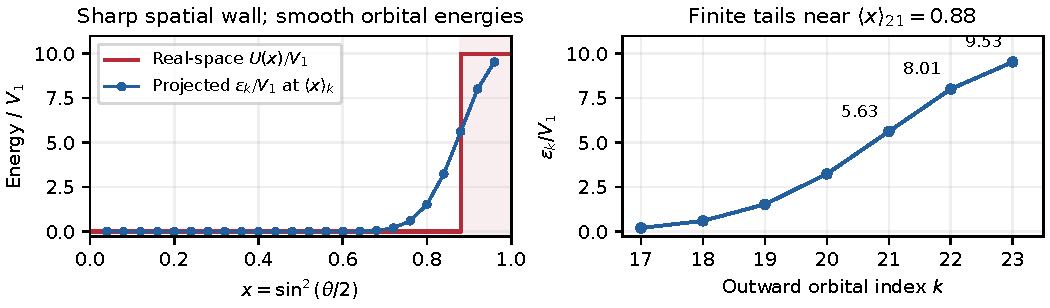
\includegraphics[width=0.89\textwidth]{wall_profile.pdf}\\[-3pt]
{\footnotesize Figure 1. $N=8$ example of the common sharp spatial wall and smooth projected energies.}
\end{center}

\textbf{Common numerical method.} Both sizes use a width-64, one-hidden-layer tanh network with complex log amplitudes. Sampling targets $q_T\propto|\psi|^{2/T}$ at $T=2$, with normalized importance weights, two sweeps per update, and uniform-sector independence proposals every 25 updates. SPRING damping is 0.001 and memory is 0.9. ED is used only to evaluate frozen checkpoints over the complete sector, never as training labels or a training matrix.

\clearpage
\begin{center}{\Large\bfseries N=8 Results and No-Edge Comparison}\end{center}

\topic{3. Exact results and controlled comparisons}
Define $\fid=|\langle\psi_0|\psi_{\rm NN}\rangle|^2$, $\de=E-E_0$, and variance $\langle(H-E)^2\rangle$, using \emph{each Hamiltonian's own} target. The $N=8$ edge target has $E_0=1.37788386\V$ and gap $0.21027795\V$; the unconfined cap has $E_0\simeq0$ and gap $0.51927662\V$. Their mutual fidelity is only $0.336144$. Confinement changes the target, and its improvement cannot be attributed to a larger sector gap. The learning rate is 0.03 throughout this table; $\rho$ bounds the parameter-update norm.

\begin{center}\small\setlength{\tabcolsep}{5pt}
\begin{tabular}{@{}lrrrrrr@{}}
\toprule
Run / endpoint & Total step & $B$ & $\rho$ & $\fid$ (\%) & $\de/\V$ & Variance$/\V^2$\\
\midrule
No edge, matched cap & 20,000 & 128 & 0.1 & $3.79\!\times\!10^{-7}$ & 0.707629 & 0.245950\\
Edge, matched cap & 20,000 & 128 & 0.1 & 84.5887 & 0.163507 & 0.399852\\
Edge, long continuation & 241,540 & 128 & 0.1 & 89.1652 & 0.128386 & 0.349859\\
Edge, radius control & 250,000 & 128 & 0.1 & 88.6466 & 0.134036 & 0.356151\\
Edge, smaller radius & 250,000 & 128 & 0.01 & 91.8694 & 0.094301 & 0.256679\\
Edge, finer radius & 270,000 & 128 & 0.001 & 92.0937 & 0.091040 & 0.248625\\
Edge, batch control & 290,000 & 128 & 0.001 & 92.0704 & 0.091074 & 0.248341\\
Edge, doubled batch & 290,000 & 256 & 0.001 & 92.3976 & 0.086664 & 0.235743\\
\textbf{Edge, 512 continuation} & \textbf{300,000} & \textbf{512} & \textbf{0.001} & \textbf{92.7420} & \textbf{0.081474} & \textbf{0.220588}\\
\bottomrule
\end{tabular}\\[3pt]
{\footnotesize Exact complete-sector diagnostics. These are the previously tabulated $N=8$ studies through batch 512.}
\end{center}

\textbf{Matched no-edge comparison.} The first two rows share fresh weights, seed, geometry and optimizer settings; 20,000 updates cost 161--162 active seconds on the RTX 4070 Ti SUPER. The unconfined trajectory places 99.73\% of probability on configurations occupying $k\ge22$, absent in the exact compact cap. The wall suppresses this escape while changing the target; the two fidelities concern different states.

\textbf{Earlier full-sphere no-edge result.} At $F=21$, $L_z=0$, the earlier 20,000-update runs reached 29.74--31.13\% fidelity and errors $0.67197$--$0.68433\V$. Their 22-input, 1,602-parameter model has 8,512 sector states: this is context, not a matched flux-23 benchmark.

The radius-0.1/0.01 branches start from the same full 230,000-update state. The finer-radius pair starts at 250,000; its $\rho=0.001$ endpoint becomes the 270,000-update origin of the matched $B=128,256$ pair. At equal 2.56 million sampled rows, $B=256$ after 10,000 updates gives $\de=0.087153\V$, versus $0.091074\V$ for $B=128$ after 20,000, at about 162 seconds each. Batch 512 then continues the 256 endpoint for 10,000 updates in 418.5 seconds, reducing error by 5.99\%. That row includes further training, without a new matched batch control.

\topic{4. Why convergence remains incomplete}
\textbf{A broadened projected edge profile and small batches are possible contributors.} The spatial wall itself is sharp; LLL projection broadens the orbital energies. At $k=21$, 56.25\% of orbital density lies beyond the step. Its causal role has not been tested against another profile. The earlier radius-0.01 endpoint actually has less density outside the wall than the exact target (0.05552 versus 0.06699 particles), so excessive leakage is not its observed failure.

The matched $B=128,256$ test supports finite-batch effects in one trajectory. Late-window median importance-weight ESS is 43.52/128 and 82.97/256, versus 179.36/512 in the later continuation. These measure weight concentration without autocorrelation correction. Both the force and metric estimates change with batch size; stochastic-gradient variance has not been measured directly.

Smaller radii reduce oscillations: six late errors span $0.0936245$--$0.0946898\V$ for $\rho=0.01$, versus $0.126928$--$0.137769\V$ for $\rho=0.1$. At the former endpoint, interaction and wall force norms 0.57260 and 0.56821 nearly cancel (cosine $-0.99374$, sum norm 0.06400), making their total demanding to estimate. Neither these correlated observations nor a plateau establish a network-capacity limit.

The batch-512 endpoint has $E=1.45935775\V$. No tabulated state meets $\fid\ge0.99$ and $\de/\mathrm{gap}\le0.01$ at three successive saved checkpoints. Resolving causes requires matched sampling, damping and step-size comparisons; every changed wall Hamiltonian needs its own exact reference.

\clearpage
\begin{center}{\Large\bfseries N=10 Results through 130,000 Updates}\end{center}

\topic{5. Larger sector, fresh network, and exact target}
The $N=10$, $F=29$, $K=135$, $L_z=10$ run starts from fresh parameters (initialization seed 7; sampling seed 71), without transferring $N=8$ weights. The same wall, $\alpha=0$, and all 30 orbitals are retained. Its exact 473,259-state sector target has
\[
E_0=1.8446958725\V,\qquad \mathrm{gap}=0.1697266664\V.
\]
The radius is $\rho=0.001$ throughout. Batch 256 and learning rate $\eta=0.03$ are used through 120,000 updates; the final 10,000-update branch uses $B=300$, $\eta=3\times10^{-5}$. All continuations retain parameters, SPRING memory/counters and training RNG states. The last branch preserves its original 256 walkers and appends 44 separately warmed chains.

\begin{center}\small\setlength{\tabcolsep}{4.5pt}
\begin{tabular}{@{}rrrrrrrr@{}}
\toprule
Total updates & $B$ & $\eta$ & $E/\V$ & $\de/\V$ & $\fid$ (\%) & Variance$/\V^2$ & Active min.\\
\midrule
0 & 256 & $0.03$ & 20.074781 & 18.230085 & $3.47\!\times\!10^{-5}$ & 31.196832 & 0.00\\
2,000 & 256 & $0.03$ & 18.047236 & 16.202540 & $8.39\!\times\!10^{-5}$ & 28.825636 & 0.67\\
10,000 & 256 & $0.03$ & 7.765967 & 5.921271 & 0.09631 & 5.815692 & 3.32\\
20,000 & 256 & $0.03$ & 5.071593 & 3.226898 & 1.66170 & 2.787697 & 6.61\\
40,000 & 256 & $0.03$ & 3.441233 & 1.596537 & 11.67139 & 1.493403 & 13.24\\
80,000 & 256 & $0.03$ & 2.525439 & 0.680743 & 45.19566 & 0.910707 & 26.53\\
120,000 & 256 & $0.03$ & 2.389667 & 0.544972 & 56.48021 & 0.891535 & 39.80\\
\textbf{130,000} & \textbf{300} & {\boldmath $3\!\times\!10^{-5}$} & \textbf{2.381588} & \textbf{0.536892} & \textbf{57.07037} & \textbf{0.882440} & \textbf{43.98}\\
\bottomrule
\end{tabular}
\\[3pt]
{\footnotesize Fidelity is percent; active minutes are cumulative, excluding compilation, warmup and evaluation.}
\end{center}

\begin{center}
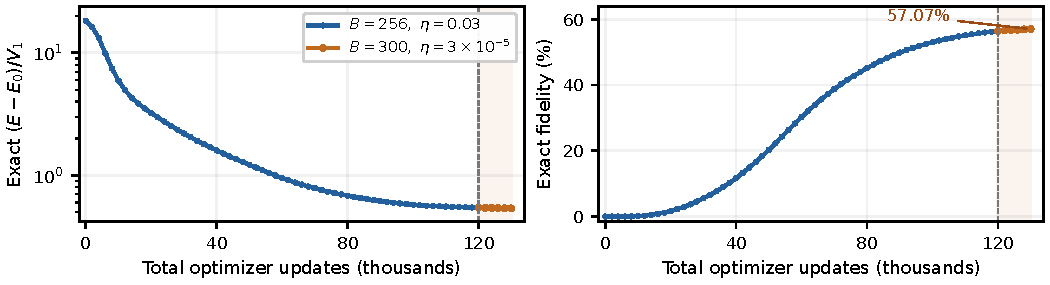
\includegraphics[width=0.96\textwidth]{n10_convergence.pdf}\\[-3pt]
{\footnotesize Figure 2. Complete-sector $N=10$ evaluations; the orange branch changes both $B$ and $\eta$.}
\end{center}

\topic{6. Outcome and interpretation}
The final branch reduces error by 1.48\% and increases fidelity by 0.59015 percentage points in 251.0 active seconds (4.18 minutes). Its median update norm is $0.00045536$, versus the preceding $0.001$. SPRING scales the raw direction by $s=\min(\eta,\rho/(\|\delta\|+10^{-8}))$; all 100 logged new updates are learning-rate limited. Using $\eta=0.01$ would still cap the initial direction. Batch and learning rate change together, so no separate benefit or speedup is established.

Saved energy and fidelity improve throughout, but variance is not monotone: it reaches $0.865393\V^2$ at 102,000 updates, then rises to $0.891535\V^2$ at 120,000. Final variance is $0.882440\V^2$ and weight ESS is about 76/300. Quantum-state variance is distinct from force-estimator noise. Final fidelity 57.07\% and $\de=0.536892\V$ fail the ground-state criterion.

\textbf{Comparison scope.} The $N=8$ batch-512 endpoint has 92.74\% fidelity and $\de=0.081474\V$, but differs in sector, network size, trajectory and update settings. The $N=10$ sector is about 30 times larger, and its spatial wall is not rescaled to the compact edge. Without an $N=10$ no-edge control, these data isolate neither particle-number nor confinement effects. Small batches, projected-edge broadening and limited expressivity remain hypotheses.

\topic{Local evidence and reproducibility}
{\footnotesize Companion manifests \path{n8_edge_note/note_evidence.json} and \path{n8_edge_note/n10_note_evidence.json} freeze source paths, exact evaluations and checkpoint hashes for every table row and plotted point. Their figure builders launch no training; the companion README gives reproduction and PDF build commands. Experiment archives remain unchanged.}
\end{document}
